\documentclass[final]{IEEEphot}

\usepackage{Socialst}
\renewcommand{\baselinestretch}{1.2} 
\jvol{xx}
\jnum{xx}
\jmonth{May}
\pubyear{2018}

\begin{document}

\title{Precise Machine Learning}

\author{Tae-Geun, Kim}

\affil{\textbf{M.S.}: Dept of Physics, Yonsei University \\
\textbf{B.S.}: Dept of Astronomy, Yonsei University }

\maketitle


\begin{abstract}
    이제 머신러닝은 거의 대부분의 이공계인들 (뿐만 아니라 문과생들에게도) 필수적인 도구가 되었습니다. 
    arXiv만 봐도 매일 머신러닝 관련 논문이 분야를 가리지 않고 나오며 페이스북에는 수 많은 머신러닝 강좌 홍보글들이 쏟아지고 있습니다. 
    개발자들 사이에서도 이제 머신러닝은 필수적인 기술 스택이 되었습니다. 따라서 머신러닝을 공부하는 것은 이제 필수불가결한 일인데, 크게 머신러닝에 접근하는 방법은 세 가지로 나눌 수 있습니다. 하나는 Developer's route 로 간단히 사람들이 만들어 놓은 Framework들을 이용해 연구에 활용하는 것입니다. 
    이 방법은 누구나 쉽게 접근할 수 있다는 장점이 있지만, 여기에 안주하다간 간단한 ML 논문 하나 읽기도 벅찰 것입니다. 
    두 번째는 Statistician's route 로 충분히 통계적 Background를 쌓은 후 Machine Learning을 이해하는 것입니다. 
    공부하는데 시간이 꽤 걸리지만 습득한 통계적 기술들은 모든 곳에 유용하게 쓰일 수 있습니다. 더불어 계속 쏟아져 나오는 ML의 신 기술들을 받아들이기도 쉽습니다. 
    마지막은 Mathematician's route 입니다. 본래 확률론은 수학의  영역입니다. 따라서 통계학의 본질에는 항상 수학이 빠질 수 없습니다. 
    비유를 하자면 통계학이 ML의 Front-end라면 수학은 ML의 Back-end인 셈이죠. 
    딱히 수학을 배운다고 실용적인 ML에 도움이 되는 것은 아닙니다만 통계에서 받아들이고 넘어가던 것에 대해 당위성을 얻게 됩니다. 
    본질적인 이해는 활용에도 도움되는 것은 당연하니 결과적으로는 좋은 영향을 미칠 것입니다. 이 문서는 마지막 방법인 Mathematician's route를 차용하여 머신러닝을 설명할 것입니다. 
\end{abstract}

\tableofcontents

\newpage

\section[Introduction]{Introduction}

\HS 우리는 자연을 관측하여 그것을 어떠한 논리를 이용하여 정해진 모델로 분류합니다. 이를 수학으로 표현하면 다음과 같습니다.

\begin{itemize}
    \item Observation: $x \in \mathbb{R}^d$
    \item Class: $y \in \{1,2,\cdots,M\}$
    \item Classifier: $g: \mathbb{R}^d \rightarrow \{1,2,\cdots,M\}$
    \item Error: When $g(x) \neq y$
\end{itemize}

\HS 우리의 목적은 관측값을 모델로 분류하는 분류기인  $g$​를 찾는 것입니다. 
당연하게도 모든 상황에 통용되는  $g$​를 찾을 수 있으면 좋겠지만 안타깝게도 그런 ​ $g$​는 존재하지 않습니다. 
하나의 관측 값이 항상 하나의 모델에만 대응되는 것은 아니기 때문이죠. 따라서 분류기에는 항상 error가 존재하기 마련입니다. 
즉, 우리의 관측은 비결정론적(Undeterministic)이고 이를 표현하기 위해서는 데카르트의 결정론적 수학을 넘어서야 합니다. 
우리는 이러한 이론을  \textbf{확률론}(Probabilistic Theory)이라 부릅니다.

\VS

\HS 확률론을 사용하기 위하여 단순히 일차원적 변수를 넘어서 하나의 쌍을 메인 변수로 볼 것입니다. 
그리고 이제 Error의 정도를 확률을 사용하여 명시할 수 있습니다. 이를 역시 수학으로 기술하면 다음과 같습니다.

\begin{itemize}
    \item Pair: $(X,Y) \in \mathbb{R}^d \times \{1,\cdots,M\}$
    \item Probability of Error: $L(g) = \P\{g(X)\neq Y\}$
\end{itemize}

그리고 이를 활용해 가장 좋은 (완벽하진 않습니다.) 분류기를 정의할 수도 있습니다.

\begin{equation}
    g^* = \argmin_{g:\mathbb{R}^d \rightarrow \{1,\cdots,M\}} L(g)
\end{equation}

이론 상 완벽하지만, 안타깝게도 우리에겐 $(X,Y)$의 분포나 $g$의 값이 주어져 있지 않습니다.
따라서 당연하게도 가장 좋은 분류기 조차 구할 수 없죠. 그렇다면 포기해야 할까요?
다행히 인류는 지금 껏 아주 많은 데이터를 생산했고 우리의 선조들은 그것을 이미 분류해놓았습니다.
우리는 지금까지 누적된 훌륭한 데이터 셋을 이용할 것입니다. 이미 분류되어 있는 데이터 셋들을 이용하면 분류기를 만들 수 있습니다. 또한, 좀 더 간편하게 데이터를 해석하기 위하여 \textit{independent identically distributed}($i.i.d$) 가정을 이용할 것입니다. 이는 비록 엄청 강력한 가정이긴 하나, 수 많은 연구에서 그리 큰 차이를 만들지 않는다는 결론을 내놓은 바 있습니다.
이제 이를 다시 수학으로 기술하여 봅시다.

\begin{itemize}
 \item Pre-Classified Data: $\{(X_i, Y_i)\}^n_{i=1}$
 \item Classifier (Trained): $g_n: \R^d\times \left(\R^d \times \M\right )^n \rightarrow \M$
 \item Conditional Probability of Error: $L_n = L(g_n) = \P\{g_n(X; \Data)\neq Y | \Data \}$
 \item Average of $L_n$: $\E  L_n$
\end{itemize}

위에서도 한 번 언급했지만 우리는 이제 분류기를 데이터 셋들로 훈련시킬 수 있습니다. 따라서 $g_n$의 차원이 상당히 복잡하죠. 
우리는 어디까지나 통계적으로 접근할 것이므로 개개인의 Error는 중요하지 않고 평균이 상당히 중요해집니다. 따라서 $\E L_n$을 사용할 것이고 이것으로 Classifier의 성능을 평가할 것입니다. 

\HS 이제 기초에 대한 수학적 서술은 대강 끝났습니다. 우리의 목표는 $\E L_n$을 최소화 시키는 것입니다. 이를 위해 우리는 확률론을 사용할텐데 확률론을 공부하기 위해서는 필수로 공부해야 하는 학문이 있습니다. 바로 \textbf{측도론}(Measure Theory)입니다.

\newpage

\section[Measure Theory]{Measure Theory} 

측도론이란, 아주 간단히 말하면 집합의 크기를 측정하기 위한 학문입니다. 우리가 보통 확률을 처음 접할 때, 다음과 같은 정의를 본 적이 있을 겁니다.

\begin{example}[High School Probability]
 Probability of occurrence of events $A$ in sample space $\Omega$ is
 \begin{equation*}
  P(A) = \frac{n(A)}{n(\Omega)}
 \end{equation*}
 \HL
\end{example}

위의 정의를 이용하면 아주 간단명료하게 확률을 구할 수 있습니다. 주사위를 던졌을 때, 1이 나올 확률은 $\{1,2,3,4,5,6\}$을 전체집합으로 설정하면 전체 6개 중에 1은 1개이기에 확률은 $\frac{1}{6}$이 됩니다. 하지만 다음의 경우에는 난처해집니다.

\begin{example}[Common High School Problem]
 정사각형 과녁 안에 원 모양 과녁이 네 변에 모두 내접하여 있을 때, 화살이 원 안에 명중할 확률을 구하여라.
 
 \HL
\end{example}

간단한 확률 지식이 있는 사람이라면 이 문제를 $\frac{\text{원의 넓이}}{\text{전체 정사각형의 넓이}}$로 접근하여 $\frac{\pi}{4}$임을 알아낼 수 있을 것입니다. 그런데 아까 분명 확률을 사건의 경우의 수를 전체 경우의 수로 나누어 구한다고 했는데 여기서 전체 경우의 수는 얼마일까요? 하다 못해 원의 경우의 수는 어떻게 구해야 할까요? 우리는 지금까지 아무런 의심 없이 구해왔습니다만, 이제부터 의심을 가져야 합니다. 확률은 특정한 경우에는 경우의 수로 구해질 수 있습니다만, 집합이 무한해지는 순간 우리가 정의한 확률은 아무 의미 없어 집니다. 따라서 우리는 확률을 엄밀하게 정의해야 할 필요가 있습니다. 그리고 그러기 위해서는 먼저 집합의 크기를 정의해야 하는 것이 우선입니다. 따라서 측도론이 필요한 것이죠.


\HS 필요성은 알았으나 측도론은 상당히 추상적인 학문이라 곧바로 집합의 크기를 어떻다 정의내릴 수 없습니다. 따라서 크기를 어떻게 정의하는지는 모르지만 측정 가능성에 대해 먼저 논해봅시다. 어떤 집합 $U, V$가 크기를 잴 수 있는 집합(가측집합; Measurable Set)이라 해봅시다. 그렇다면 직관적으로 다음의 사실들을 받아 들일 수 있습니다.

\begin{itemize}
 \item $U\cup V$ is measurable
 \item $U\cap V$ is measurable
 \item $U^c,~ V^c$ is measurable
\end{itemize}

하지만 수학자들은 이런 모호한 직관의 정렬을 좋아하지 않습니다. 이런 규칙들을 모아 하나의 우아한 규칙으로 정의내리죠. 수학에서 이러한 규칙을 우리는 대수(Algebra)라고 부릅니다. 

\newpage

\begin{definition}[$\sigma$-algebra]
 Let $S$ be a set, and let $\F$ be a family of subsets of $S$. $\F$ is called a $\sigma$-algebra if
 
 i) $\emptyset \in \F$
 
 ii) $A\in\F$ implies $A^c \in \F$

 iii) $A_1,A_2,\cdots \in \F$ implies $\displaystyle \bigcup_{i=1}^{\infty} A_i \in \F$

 \HL
 \end{definition}

 정의는 무척 복잡해보이지만, 사실 의미는 간단합니다.  대수는 일종의 규칙을 담아 놓은 집합입니다. 예를 들어 위상수학에서의 Topology는 모든 열린 집합들의 집합이며 여기서 말하는 $\sigma$-algebra(시그마대수)는 모든 가측집합들의 집합입니다. 공집합은 너무나 당연하게 그 크기를 0으로 측정할 수 있을 테고 어떤 집합 $A$가 측정 가능하다면 (이를 수학에서 $A\in \F$라고 표현하는 겁니다.) 그의 여집합 또한 측정할 수 있어야 할 것입니다. 마지막으로 측정 가능한 집합들을 무한히 합친다해도 그 역시 측정 가능할 것 입니다. 이를 단순히 수학이라는 언어로 기술한 것에 지나지 않습니다. 또한 수학의 함축성으로 인해 정의를 대폭 줄일 수 있었습니다.  위의 정의에서 i), ii) 정의를 이용하면 전체 집합 역시 측정가능하다는 것을 알 수 있고 ii), iii) 을 이용하면 합집합들 뿐 아니라 교집합들 역시 측정 가능하다는 사실을 알 수 있습니다. 
 
 \HS 대수는 일종의 규칙이라 하였는데, 따라서 대수가 있는 공간과 아닌 공간은 구별되어야 합니다. 따라서 우리는 이를 다음과 같이 수학적으로 정의합니다.
 
  \begin{definition}[Measurable Space]
    Let $S$ be a set, and let $\F$ be a $\sigma$-algebra of subsets of $S$. Then $(S, \F)$ is called a measurable space. The elements of $\F$ are called measurable sets.
    
    \HL
 \end{definition}

이제 대략적인 Notation은 정리했으니 조금 더 생각을 해봅시다. 어떤 집합 $S$에 대하여 가장 작은 $\sigma$-algebra와 가장 큰 $\sigma$-algebra는 뭘까요? 일단, 정의에 의해 공집합은 무조건 측정가능하고 두 번째 정의에 의해 전체집합도 측정가능하므로 가장 작은 시그마대수는 $\F = \{\emptyset, S\}$가 됩니다. 또한 시그마 대수는 어떤 집합의 부분집합의 모임이기 때문에 모든 부분집합의 집합(멱집합; Power set)이 가장 큰 시그마 대수가 될 것입니다. 이는 $\F = \mathcal{P}(S)$로 표기합니다.

고등학교 시절에 부분집합을 배울 때, 어떤 집합을 포함하는 부분집합의 개수는? 이라는 문제를 본 적이 있을 겁니다. 되게 의미 없는 일 같지만 수학에서는 어떤 집합을 포함하고 있는 지의 여부가 상당히 중요합니다. 시그마 대수에서도 마찬가지인데 어떤 집합을 반드시 포함하고 있는 시그마 대수를 "그 집합에 의하여 발생한 시그마 대수이다" 라고 정의할 것입니다. 수학적 정의는 다음과 같습니다.

\begin{definition}
 Let $S$ be a set and $G$ be a family of subsets of $S$. The smallest $\sigma$-algebra which contains $G$ is called generated $\sigma$-algebra with respect to $G$ denoted by $\sigma(G)$.
 
 \HL
\end{definition}

 이제 이 정의를 아주 유명한 규칙 공간에 이용해보겠습니다. 바로 위상공간(Topological Space)에 말이죠.
 
 \newpage

 \begin{definition}[Borel $\sigma$-algebra]
  The Borel $\sigma$-algebra $\B$ of a topological space $(S,\mathcal{T})$ is the $\sigma$-algebra generated by $\mathcal{T}$.

  \HL
 \end{definition}

이 정의를 이해하기 위하여 굳이 위상수학까지 공부하지 않아도 됩니다. 우리는 앞으로 관측 공간인 $\R^d$에서의 대수만 사용할 것이기 때문이죠. 간단히 말하자면 $n$차원 실수공간의 위상은 $n$차원 직육면체로 표현됩니다. 1차원에서는 직선, 2차원에서는 직사각형 이런 식이죠. 따라서 위의 정의에 따르면 이런 직사각형들이 모두 측정가능하다면 그 공간을 일컬어 Borel $\sigma$-algebra 가 존재하는 공간이라 합니다. 

지금까지는 공간, 집합에 대해서만 다뤘는데 우리의 가장 중요한 것은 그 공간에 작용하는 함수입니다. 위상수학이나 해석학을 했다면 다음의 정의는 아주 쉽게 다가올 것입니다. 만일, 하지 않았더라도 받아들이면 됩니다.

\begin{definition}[Measurable function]
 Let $(S, \F),~(S',\F')$ be measurable spaces and $f\,:\,S \rightarrow S'$. If $\forall X \in \F'$, $f^{-1}(X) \in \F$ then $f$ is called measurable function.
 
 \HL
\end{definition}

이 정의를 어떻게 사용하는지 간단한 예시를 들어 설명해보겠습니다.

\begin{definition}[Indicator Function]
 The indicator function of a subset $A$ of a set $X$ is a function 
 
 \begin{equation*}
    I_A(x)\,:\,X \rightarrow \{0,1\}
 \end{equation*}
 
defined as

\begin{equation*}
 I_A(x) := \begin{cases}1&{\text{if }}x\in A,\\0&{\text{if }}x\notin A.\end{cases}
\end{equation*}

\HL
\end{definition}

\begin{example}[Indicator function is measurable]
 Let $A \in \F$ then $I_A$ is measurable function.
 
 \HL
\end{example}

 위의 예시의 증명은 아주 간단하므로 생략하겠습니다. 꼭 한 번 해보고 넘어가면 이해가 잘 될테니 꼭 해보시길 바랍니다. 이제 측정가능성은 대부분 논의했으니 우리의 진정한 목표인 측도로 가봅시다.

\newpage

\begin{definition}[Measure]
 Let $(S, \F)$ be measurable space and let $\mu\,:\, \F \rightarrow [0,\infty)$ be a function. $\mu$ is measure on $\F$ if
 
 i) $\mu(\emptyset) = 0$
 
 ii) $\mu$ is $\sigma$-additive. That is, for disjoint family $\{A_i\}_{i=1}^\infty \in \F, $
 
 \begin{equation*}
  \mu\Sbk{\bigcup_{i=1}^\infty A_i} = \sum_{i=1}^\infty \mu(A_i)
 \end{equation*}

 \HL
\end{definition}

정의는 아주 자명합니다. 비록 크기가 무엇인지 감이 잘 오진 않더라도 공집합의 크기는 반드시 0일 것이며 전혀 겹치지 않는 집합들의 합집합의 크기는 각 집합들의 크기의 합과 같을 것입니다. 또한 위 정의에서 유심히 보아야 할 부분은 $\mu$ 즉, 측도가 측정가능한 집합을 음이 아닌 값의 실수로 보내는 함수라는 것입니다. 우리는 음의 부피를 정의하지 않고 또한 음의 확률을 정의하지 않습니다. 사실 너무나 당연하게 써 왔던 이러한 사실을 측도라는 비교적 간단한 정의를 이용하여 수학적으로 못 박아 둔 것이죠.   이제 측도도 생겼으니 새로운 공간을 정의하여 봅시다.

\begin{definition}
 The triple $(S,\F,\mu)$ is a measure space if $(S,\F)$ is a measurable space and $\mu$ is a measure on $\F$.
 
 \HL
\end{definition}

순수 수학자들이 아닌 이상 응용수학이나 물리, 통계학에서는 측정 가능성도 꽤 중요하겠지만 더욱 중요한 것은 정확히 측정하는 것입니다. 따라서 이제부터는 새로 정의한 측도공간(Measure Space)을 사용할 것입니다. 이러한 측도 공간에서도 $n$차원 실수 공간은 특히 더욱 중요해서 따로 이름을 붙입니다.

\begin{definition}[Lebesgue Measure]
 The \textbf{Lebesgue measure} $\lambda$ on $\R^d$ is a measure on the Borel $\sigma$-algebra of $\R^d$ such that the $\lambda$ measure of each rectangle equals to its volume.
 
 \HL
\end{definition}

정의는 조금 복잡할지라도 의미는 간단합니다. 직육면체의 부피를 측정하는 측도를 \textbf{르벡 측도(Lebesgue measure)}라고 부른다는 것이죠. Lebesgue의 이름은 수학 어디서나 등장하기 때문에 익숙해지는 것이 좋습니다.
이제 측도도 생겼으니 본격적으로 집합의 크기를 측정해봅시다. 물론, 처음부터 복잡한 함수로 표현되는 공간의 크기를 구하기란 아주 어려운 일이므로, 우리는 아주 단순한 함수부터 시작해서 일반화하는 방향으로 접근할 것입니다.

\newpage

\begin{definition}[Simple Function]
	A function, which image is finite, is called simple function.
	
	\HL
\end{definition}

\begin{property}[Simple function with Indicator function]
	\label{prop:1}
	If $\varphi:\chi \rightarrow \R$ is simple function then we can write 
	$$\varphi = \sum_{i=1}^{n}a_iI_{E_i}$$ 
	where $\{a_i\}$ is image of $\varphi$ and $E_i = \varphi^{-1}(\{a_i\})$.
	
	\HL
\end{property}

수학에서 사용되는 전형적인 단순한 함수는 바로 위에서 정의한 Simple function입니다. 사실 본래 정의는 매우 간단하지만, 보통 Simple function이라 하면 대개 Property~\ref{prop:1}을 생각합니다. 대체 이 함수가 뭐가 단순한건지 의아하겠지만, 이러한 함수에 대해서는 적분을 아주 쉽게 정의할 수 있습니다.

\begin{definition}[Lebesgue Integral for Simple function]
	Let $(S,\F, \mu)$ be measure space and $\displaystyle f = \sum_{i=1}^{n}a_i I_{E_i}$ be a simple function. Then the \textbf{Lebesgue Integral} of $f$ with respect to $\mu$ is defined by
	$$ \int_S f d\mu = \sum_{i=1}^{n}a_i \mu(E_i)$$
	
	\HL
\end{definition}

분명 정의는 했는데 대체 무슨 뜻인가 싶을 수 있으니 한 번 쉽게 예시를 들어봅시다.

\begin{example}[Example of Lebesgue Integral for simple function]
	$f$ is a simple function given as:
	
	$$ f =
	\begin{cases}
		1 & \text{if}~ 0 \leq x < 1 \\
		2 & \text{if}~ 1 \leq x < 3 \\
		3 & \text{if}~ 3 \leq x < 4 \\
		0 & \text{otherwise}
	\end{cases}
	$$
	
	then find integral of $f$ in $\R$.
	
	\HL
\end{example}

이 문제는 직사각형의 넓이만 구할 수 있으면 쉽게 구할 수 있습니다.

\newpage

일단 이 함수는 다음과 같이 그려집니다.

\begin{figure}[h!]
	\centering
	\begin{subfigure}{.6\textwidth}
		\centering
		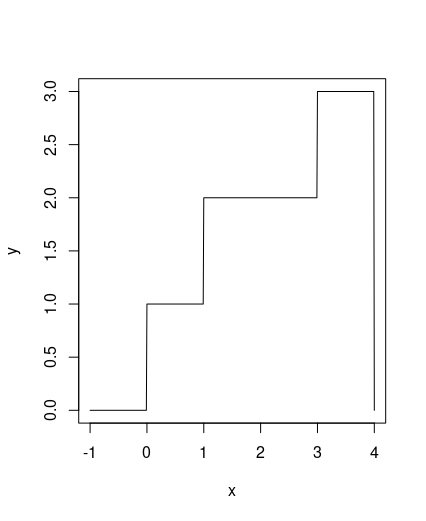
\includegraphics[width=\textwidth, height=9.5cm]{simple.png}
	\end{subfigure}
	\caption{Simple Function Example}
\end{figure}

이 함수를 Indicator Function을 이용하여 식으로 구해보면 다음과 같습니다.

$$ f(x) = 1\times I_{E_1} + 2\times I_{E_2} + 3\times I_{E_3} $$

이때 $E_1,E_2,E_3$는 각각 $[0,1), \, [1, 3),\, [3,4)$입니다.
앞에서 정의했던대로 르벡 적분(Lebesgue Integral)을 이용해서 구해보면 쉽게 답을 구할 수 있습니다.

$$\int_\R f d\mu = \sum_{i=1}^{3} a_i \mu(E_i) = 1\times1 + 2\times 2 + 3\times 1 = 8$$

식을 자세히 보면 그저 직사각형의 넓이들을 더한 값과 같다는 것을 알 수 있습니다. 이렇게보면 굳이 쉬운 문제를 어렵게 푸는 것 같아 보이지만, 르벡 적분의 의의는 이런 단순한 함수 뿐만 아니라, 무한한 집합이나 추상적인 집합에 대해서도 적분 값을 구할 수 있다는 것입니다.

\VS

\HS 항상 이런 단순한 정의로 문제를 풀 수 있으면 좋겠지만 대다수의 경우에 함수들은 Simple function으로 나타낼 수 없습니다. (간단히 연속함수의 예시만 봐도 알 수 있죠.) 따라서 우리는 기존 정의를 확장해야할 필요가 있습니다.

\newpage

\begin{definition}[Lebesgue Integral for Positive definite function]
	Let $(S, \F, \mu)$ be a measure space and $f: S \rightarrow [0,\infty)$ is measurable, then the Lebesgue Integral of f with respect to $\mu$ is defined by
	$$ \int_S f d\mu = \sup\Mbk{\int_S \varphi d\mu : \varphi\text{ is simple and measurable, } 0 \leq \varphi \leq f }$$
	
	\HL
\end{definition}

위 정의를 보면 앞에서 왜 Simple Function을 도입해야 했는 지 이해가 됩니다. 마치 리만 적분(Riemann Integral)에서 작은 직사각형들로 잘게 쪼개어 적분을 표현하듯이 르벡 적분에서는 함수를 Simple Function으로 열심히 쪼개어 적분합니다. 백문이 불여일견이니 그림으로 보면 이해가 쉬울 겁니다.

\begin{figure}[h!]
	\centering
	\begin{subfigure}{.8\textwidth}
		\centering
		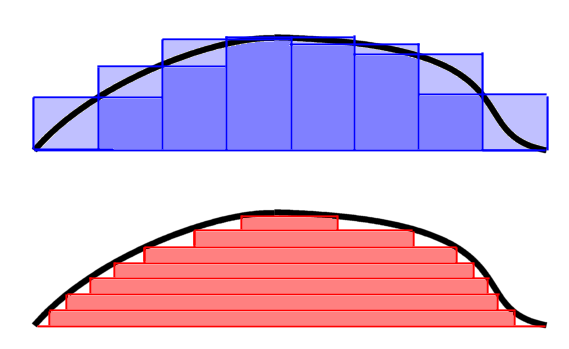
\includegraphics[width=\textwidth, height=9.5cm]{riemann_vs_lebesgue.png}
	\end{subfigure}
	\caption{Riemann vs Lebesgue}
\end{figure}

물론 양의 함수만 있는 것은 아니니 음의 함수까지도 정의를 확장해야 합니다.

\begin{definition}[Lebesgue Integral for Arbitrary Measurable Function]
	Let $(S, \F, \mu)$ be a measure space and $f: S\rightarrow \R$ is arbitrary measurable function. Then
	$$\int_S f d\mu = \int_S f^+ d\mu - \int_S f^- d\mu$$
	where $f^+ = \max\Mbk{f(x), 0},~f^- = \max\Mbk{-f(x),0}$.
	
	\HL 
\end{definition}

\newpage

르벡 적분의 주요 정리들:

\begin{theorem}[Beppo - Levy Theorem]
	If $f_n \rightarrow f~(mod~\mu)$ in a monotone increasing way then
	$$\int \lim_{n\rightarrow\infty}f_n d\mu = \lim_{n\rightarrow\infty}\int f_n d\mu$$
	
	\HL
\end{theorem}

\begin{theorem}[Fatou's Lemma]
	Let $(S, \F, \mu)$ be a measure space and $\forall n \in \mathbb{N}$, $f_n : S \rightarrow [0,\infty)$ be measurable function. Then
	$$\int_S \liminf_{n\rightarrow\infty}f_n d\mu \leq \liminf_{n\rightarrow\infty} \int_S f_n d\mu$$
	
	\HL
\end{theorem}

\begin{theorem}[Lebesgue Dominated Convergence Theorem]
	Let $(S,\F,\mu)$ be a measure space. Assume that $f_n \rightarrow f~(mod~\mu)$ and $|f_n(s)| \leq g(s)$, $\forall s \in S, n \in \mathbb{N}$ where $\int_S g d\mu < \infty$. Then
	$$\int_S f d\mu = \lim_{n\rightarrow\infty} \int_S f_n d\mu$$
	
	\HL
\end{theorem}

위 정리들은 수학에서는 상당히 중요한 정리지만, 지금 당장 우리에게는 많이 필요한 것은 아니니 한 번 보고 넘어가면 충분합니다.

\VS

\HS 하지만 다음 정의들과 정리들은 꽤 중요하니 눈여겨 봐두시길 바랍니다.

\begin{definition}[Induced Measure]
	Let $(S, \F, \mu)$ be a measure space and $f$ be a measurable function. Then $f$ induces a measure $\nu$ on the Borel $\sigma$-algebra $\B$
	$$\nu(B) = \mu(f^{-1}(B)),~ \forall B \in \B$$
	
	\HL
\end{definition}

\begin{theorem}[Change Measure]
	Let $\nu$ be a measure on the Borel $\sigma$-algebra of $\mathbb{R}$ and let $f,g$ be measurable functions. Then $\forall B \in \B$,
	$$\int_B g d\mu = \int_{f^{-1}(B)} g \circ f d\nu$$
	
	\HL
\end{theorem}

\newpage

\begin{definition}[Product Measure]
	Let $\nu_1,\nu_2$ be measures on $(S_1, \F_1),~(S_2, \F_2)$. Let $(S,\F)$ be measurable space such that $S = S_1\times S_2$ and $\F = F_1\times F_2$ whenever $F_1\in \F_1, ~ F_2\in \F_2$.
	$\nu$ is called the product measure of $\nu_1, \nu_2$ on $\F$ if 
	$$\nu(F_1 \times F_2) = \nu(F_1)\times \nu(F_2)$$
	
	\HL
\end{definition}

\begin{theorem}[Fubini's Theorem]
	Let $h$ be a measurable function on the product space $(S,\F)$ then
	$$\int_S h(u,v) d\mu = \int_{S_1}\Sbk{\int_{S_2} h(u,v) d\nu_2}d\nu_1 = \int_{S_2}\Sbk{\int_{S_1} h(u,v) d\nu_1}d\nu_2 $$
	
	\HL
\end{theorem}

위 정의와 정리들은 우리가 흔히 리만 적분에서 적분 변수를 변경할 때 사용했던 것과 비슷하므로 외우기는 쉬울 겁니다. 여기서는 굳이 증명이 필요치 않으니 생략하고 넘어가겠습니다.

\VS

\HS 그럼 이제 본격적으로 확률론의 세계로 들어가봅시다.

\newpage

\section{Probability Theory}

\begin{definition}[Probability Space]
	A Measure space $(\Omega, \F, \P)$ is called a probability space if $\P(\Omega) = 1$. $\Omega$ is called the sample space, the measurable sets are called events, and the measurable functions are called random variables. If $X_1,X_2,\cdots,X_n$ are random variables then $X = (X_1, X_2,\cdots,X_n)$ is a vector-valued random variable.
	
	\HL
\end{definition}

\HS 확률공간의 정의는 간단합니다. 어떤 측도공간 $(\Omega, \F, \P)$가 $\P(\Omega) = 1$을 만족할 때, 그 측도공간을 확률 공간이라 부른다는 것입니다. 또한, 전체 집합인 $\Omega$는 표본공간(Sample Space)이라 부르며 가측집합(Measurable Set)들은 사건(Events)이라 부르고 가측함수(Measurable Function)들은 확률변수(Random Variable)라고 부른다는 것이죠. 계속해서 다른 정의들을 봅시다.

\begin{definition}[Distribution of Random Variables]
	Let $X$ be a random variable, then $X$ induces the measure $\mu$ on the Borel $\sigma$-algebra of $\R$ by
	$$\mu(B) = \P \Mbk{\{\omega:~ X(\omega)\in B\}} \equiv \P \Mbk{X\in B}, ~ B \in \B$$
	The induced probability measure $\mu$ is called the distribution of random variable $X$.
	
	\HL
\end{definition}

앞에서 말한 Induced Measure가 뜬금없이 튀어나왔습니다. 하지만 굳이 Induced e 부분을 볼 필요는 없습니다. 여기서 기억해야 할 것은 $\mu(B) = \P \Mbk{X \in B}$ 입니다. 이는 우리가 아는 확률과 상당히 유사합니다. 집합 B에 확률변수 X가 들어갈 확률을 새로운 $\mu$라는 측도로 정의한 것이죠. 이때, $\mu$의 이름은 확률변수 $X$의 분포(Distribution)입니다. 즉, 확률분포를 구한다는 것은 측도 $\mu$를 구한다는 것과 동치입니다.

\VS

\HS 이제 볼 정의는 상당히 많이 쓰이므로 특히나 주의 깊게 보시길 바랍니다.

\begin{definition}[Expectation]
	Let $X$ be a random variable. The expectation of $X$ is the integral of $X$ with respect to distribution $\mu$ of $X$.
	$$ \E\{X\} = \int_\R x \mu(dx)$$
	
	\HL
\end{definition}

적분 기호가 낯설 수 있는데 이는 보통 르벡 적분에 대해서 표현하는 방식이 여러가지기 때문입니다.
$$\int_S f d\mu = \int_S f(s) \mu(ds) $$

하지만 여전히 위 정의는 이상합니다. $X$ 에 대한 기댓값이라면서 $X$가 적분식에 포함되어 있지 않습니다. 하지만 자세히 보면 $\mu$가 $X$의 분포이기에 $\mu$ 안에 $X$의 값이 포함되어 있다는 것을 알 수 있습니다.
이만 각설하고 기댓값의 정의가 나왔으니 당연하게도 분산의 정의가 등장해야곘죠.

\newpage

\begin{definition}[Variance]
	Let $X$ be a random variable. The variance of $X$ is
	$$ \Var\{X\} = \E \Mbk{(X - \E\{X\})^2}$$
	
	\HL
\end{definition}

우리가 아는 분산의 정의와 정확히 일치합니다. 즉, Measure Space로부터 복잡하게 유도되긴 했지만 실제 계산은 고등학교때 배우던 확률과 통계와 크게 다르지 않다는 것을 알 수 있습니다. 이제 또 다른 익숙한 개념을 새롭게 정의해봅시다.

\begin{definition}[Joint Distribution \& Independence]
	Let $X_1,\cdots,X_n$ be random variables. They induce the measure $\mu^{(n)}$ on the Borel $\sigma$-algebra of $\R^n$ with the property
	$$\mu^{(n)}(B_1 \times \cdots \times B_n) = \P\{X_1 \in B_1, \cdots,X_n \in B_n \}, ~ B_1,\cdots,B_n \in \B$$
	$\mu^{(n)}$ is called the \textbf{joint distribution} of random variables. Let $\mu_i$ be the distribution of $X_i$, the random variables $\{X_i\}_{i=1}^{n}$ are \textbf{independent} if $\mu^{(n)}$ is the product measure of $\{\mu_i\}_{i=1}^n$. The events $A_1, \cdots, A_n \in \F$ are independent if the random variables $I_{A_1}, \cdots, I_{A_n}$ are independent.
	
	\HL 
\end{definition}

위 정의는 한 마디로 요약하면 확률변수 $n$개의 분포가 각각의 확률변수들의 분포에 대해 곱측도(Product Measure)이면 확률변수들을 독립이라 부르겠다는 정의입니다. 우리가 알던 정의와 상당히 다른 것 같지만 확률측도로 변경하여 보면 위 정의는 다음 식으로 정리됩니다.

$$\P\{X_1 \in B_1, \cdots,X_n \in B_n \} = \P\Mbk{X_1 \in B_1} \times \cdots \times \P\Mbk{X_n \in B_n}$$

이제 우리가 아는 정의와 상당히 유사해졌습니다. 또한 위 정의는 단순히 확률 변수들의 독립 뿐만 아니라 사건들의 독립도 정의하였습니다. 특이하게도 각 사건들의 Indicator Function들이 독립이면 그 사건들도 독립이라고 정의되어 있는데 Indicator Function 역시 Measurable function이므로 확률 변수에 해당하니 정의 자체는 충분히 받아들일 수 있습니다. 위 정의를 받아들이면 아래의 중요한 정리를 쉽게 유도할 수 있습니다.

\begin{theorem}[Independence with Expectation]
	If $X_1,\cdots , X_n$ are independent and have finite expectations then
	$$ \E \Mbk{X_1X_2\cdots X_n} = \E\Mbk{X_1} \cdots \E\Mbk{X_n}$$
	
	\HL
\end{theorem}

증명은 Independence, Product Measure의 정의들과 Fubini's theorem을 적용하면 쉽게 증명되니 생략하겠습니다.

\newpage

\subsection{Inequalities}

\HS 이제 지루한 수학 단원의 마지막입니다. 앞으로 논리를 전개하는데 유용한 부등식들을 소개하고 마치도록 하겠습니다.

\VS

- Cauchy-Schwartz : $\displaystyle |\E(XY)| \leq \sqrt{\E(X^2)\E(Y^2)}$

\vs

- H{\"o}lder : $\displaystyle p,q \in (1,\infty),~\frac{1}{p} + \frac{1}{q} = 1 \Rightarrow \E(|XY|) \leq \Sbk{\E(|X^p|)}^{1/p} \cdot \Sbk{\E (|Y^q|)}^{1/q}$

\vs

- Markov : Given non-negative $X$, $\forall t > 0$, $\displaystyle \P(X\geq t) \leq \frac{\E(X)}{t}$

\vs

- Chebyshev : $\displaystyle \forall t > 0, ~\P(|X - \E X| \geq t) \leq \frac{\Var(X)}{t^2}$

\vs

- Chebyshev - Cantelli : $\displaystyle \forall t \geq 0,~ \P(X-\E X > t ) \leq \frac{\Var(X)}{\Var(X) + t^2}$

\VS

위의 부등식들도 상당히 중요하지만 다음 2개의 부등식은 특히나 중요하기에 굳이 정리로 정리하였습니다.

\begin{theorem}[Jensen's Inequality]
	If $f$ is a real-valued convex function on a finite or infinite interval of $\R$ and $X$ is a random variable with finite expectation taking its values in this interval. Then
	$$f(\E(X)) \leq \E(f(X))$$
	
	\HL
\end{theorem}

\begin{theorem}[Association Inequality]
	Let $X$ be a real-valued random variable and $f,g$ are real-valued function
	
	i) $f,g$ are monotone non-decreasing then
	$$ \E\Mbk{f(X) g(X)} \geq \E\Mbk{f(X)}\E\Mbk{g(X)}$$
	
	ii) $f$ is monotone increasing and $g$ is monotone decreasing then
	$$ \E\Mbk{f(X) g(X)} \leq \E\Mbk{f(X)}\E\Mbk{g(X)}$$
	
	\HL
\end{theorem}

그럼 이제 소소한 일탈을 마치고 다시 우리의 본분인 머신러닝으로 돌아가봅시다.
%% \ackrule

%\bibliographystyle{IEEEtran}
%\bibliography{thesis}

%\section*{Biographies}

%\textbf{P. W. Wachulak} received the degree${\ldots}$ \\[6pt]
%\textbf{M. C. Marconi} received the degree${\ldots}$ \\[6pt]
%\textbf{R. A. Bartels} received the degree${\ldots}$ \\[6pt]
%\textbf{C. S. Menoni} received the degree${\ldots}$ \\[6pt]
%\textbf{J. J. Rocca} received the degree${\ldots}$


\end{document}
